%Empieza configuracion de capitulo
\setstretch{1.0}
\titleformat{\chapter}[block]{\Large\bfseries}{CAP'ITULO \Huge\thechapter\vspace{25 pt}}{0 pt}{\\\fontsize{26}{36}\selectfont}
\titlespacing{\chapter}{0 pt}{30 pt}{50 pt}[0 pt]
\titleformat{\section}{\Large\bfseries}{\thesection}{0 pt}{\hspace{30 pt}}
\titleformat{\subsection}{\large\bfseries}{\thesubsection}{0 pt}{\hspace{30 pt}}
\pagestyle{fancy}
\fancyhead[LO,LE]{\footnotesize\textit{\leftmark}}
\fancyhead[RO,RE]{\thepage}
\fancyfoot[CO,CE]{}
%Termina configuracion de capitulo

\chapter{Planeaci'on} %Cambia al nombre de tu capitulo
\setstretch{1.5} %Regresa el interlineado a 1.5

\normalsize

\section{Cronograma}
\noindent
El cronograma mostrado a continuaci'on contiene las actividades realizadas en el transcurso del desarrollo del proyecto de tesis.\\

Se ilustra desde el descubrimiento del tema de investigaci'on hasta su posterior defensa. Cabe aclarar que todas las actividades fueron definidas, revisadas y supervisadas por el asesor de tesis.

\begin{figure}[H]
\centering
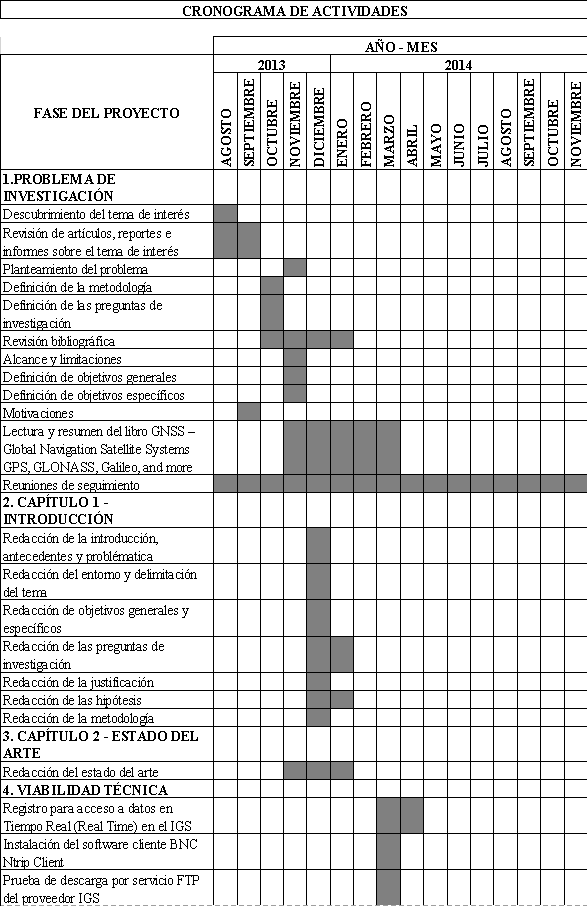
\includegraphics[width=0.95\textwidth]{images/Gantt_1}
\caption{Parte 1 - Cronograma de actividades con diagrama de Gantt}
\label{fig:3.1}
\end{figure}

\begin{figure}[H]
\centering
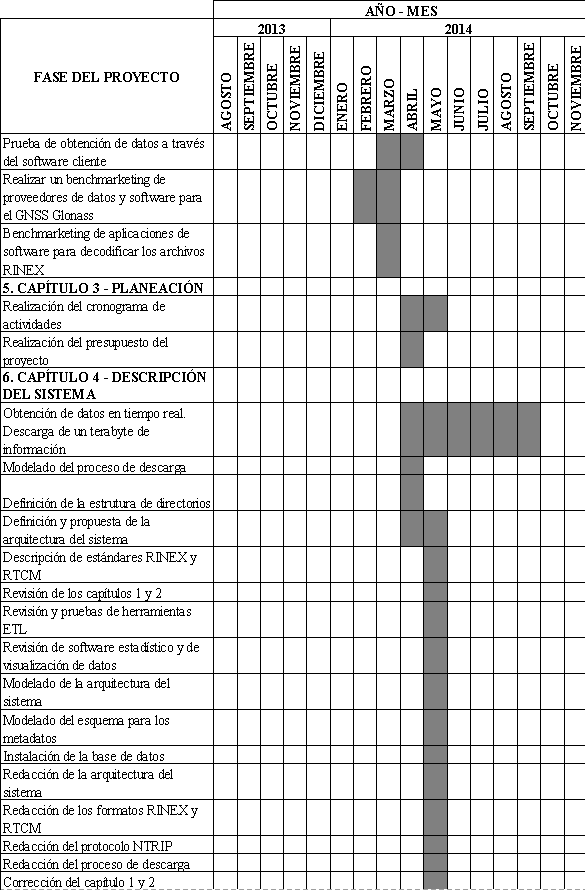
\includegraphics[width=0.95\textwidth]{images/Gantt_2}
\caption{Parte 2 - Cronograma de actividades con diagrama de Gantt}
\label{fig:3.2}
\end{figure}

\begin{figure}[H]
\centering
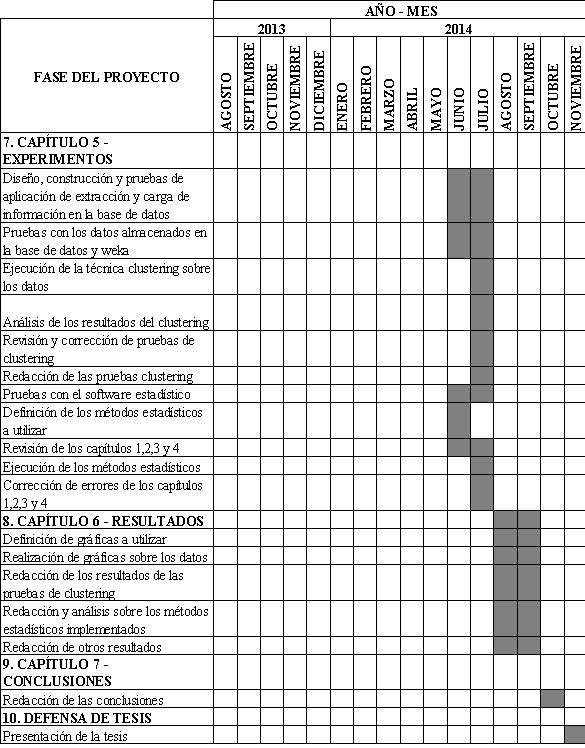
\includegraphics[width=0.95\textwidth]{images/Gantt_3}
\caption{Parte 3 - Cronograma de actividades con diagrama de Gantt}
\label{fig:3.3}
\end{figure}

\section{Presupuesto}
\noindent
A continuaci'on se presenta el presupuesto elaborado para llevar a cabo el proyecto de tesis.
La notaci'on usada para la separaci'on de miles es el car'acter punto (.).\\

\begin{figure}[H]
\centering
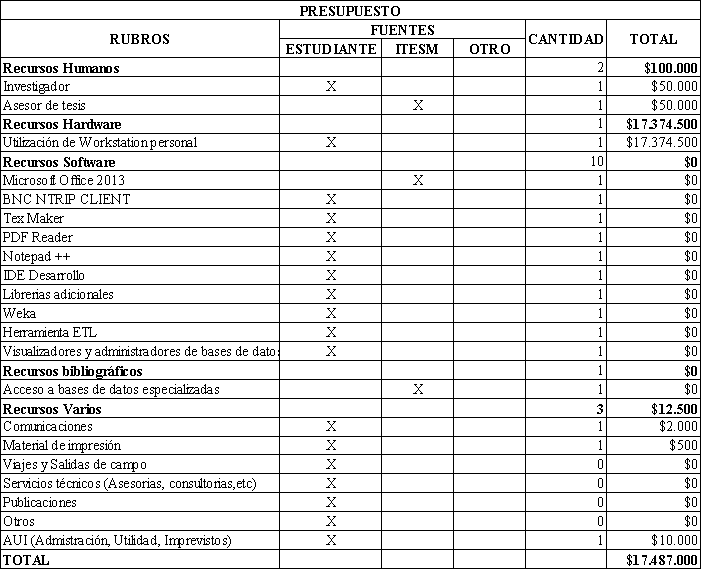
\includegraphics[width=0.95\textwidth]{images/Presupuesto}
\caption{Presupuesto del proyecto de tesis.}
\label{fig:3.4}
\end{figure}

\clearpage